Para poder enfrentarnos con garantías al desarrollo del proyecto es
necesario conocer una serie de conceptos relacionados con el sonido y
la música en general, y conceptos sobre análisis de señales que
explicaremos a lo largo de este capítulo.

\section{El sonido}
Un \textbf{sonido} es una vibración que se propaga por un medio
elástico en forma de onda. Estas vibraciones se transmiten de forma
longitudinal, esto es, en la misma dirección en la que se propaga el
sonido. El medio más común para la transmisión del sonido es el
\textbf{aire}. 

El sonido, en su forma más simple, se compone de una sola onda
sinusoidal básica, con las características tradicionales: amplitud,
frecuencia y fase.

\subsection{Frecuencia y tono}
La \textbf{frecuencia} mide el número de oscilaciones de la onda por
unidad de tiempo. Por regla general, se utiliza el \textbf{hercio}
como unidad de medida de frecuencia, que indica la cantidad de
repeticiones por segundo. La frecuencia determinará la \textbf{altura}
del sonido, es decir, cómo de grave o agudo es. Los sonidos graves
tienen una frecuencia baja, mientras que los sonidos agudos tienen una
frecuencia alta.

A lo largo de los años se ha establecido un estándar de referencia que
establece que la nota \textit{la} que se encuentra encima del
\textit{do} central del piano debe sonar a 440 hercios de
frecuencia. Esta medida se utiliza a la hora de afinar los
instrumentos, de modo que si al tocar la nota \textit{la} se detecta
un tono con una frecuencia de 440 hercios, entonces el instrumento
estará bien afinado.

El oído humano es capaz de detectar sonidos a partir de los 20
hercios. Los sonidos por debajo de esa frecuencia se conocen como
\textbf{infrasonidos}. Por otro lado, el límite auditivo en
frecuencias altas varía mucho con la edad: un adolescente puede oir
sonidos con frecuencias hasta los 18kHz, mientras que un adulto de
edad media solo suele llegar a captar sonidos de hasta 13kHz. El
límite genérico superior se establece en 20kHz, por encima de los
cuales los sonidos se denominan \textbf{ultrasonidos}.

\subsection{Amplitud}
La \textbf{amplitud} representa la energía que transporta la
onda. Cuando un instrumento u otro objeto genera una vibración, la
amplitud es la cantidad de movimiento que esa vibración genera.
Podría equipararse (de forma no estricta) a la intensidad del sonido:
cuanto mayor sea la amplitud, más fuerte se oirá el sonido.

\subsection{Fase}
Por último, la \textbf{fase} ($\varphi$) indica el desplazamiento
horizontal de la onda respecto del origen. Si la fase de una onda no
es cero, entonces parecerá que está \textit{desplazada} hacia la
derecha, si la fase es positiva, y hacia la izquierda si la fase es
negativa.

\begin{center}
  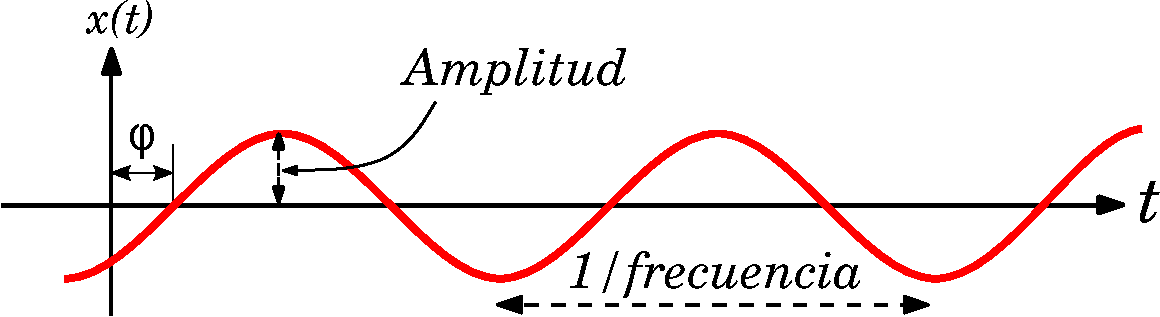
\includegraphics[scale=0.7]{conceptos/onda}  
\end{center}

\section{Descomponiendo sonidos}
Para desarrollar oFlute nos interesa conocer la altura de la nota que
está tocando la flauta en un instante concreto. Para un tono puro,
podríamos conocer la altura fijándonos en su frecuencia. El problema
es que, en la naturaleza, \textbf{no existen} los tonos puros, sino
que los sonidos se componen de multitud de tonos de diferentes
amplitudes, frecuencias y fases. 

Afortunadamente, la teoría dicta que cualquier onda periódica puede
descomponerse como suma de tonos puros de distintas frecuencias,
llamados \textbf{armónicos}. La menor de todas estas frecuencias se
conoce como \textbf{frecuencia fundamental}, y todas las otras
frecuencias son múltiplos enteros de ella. La frecuencia fundamental
es la que dicta la altura \textit{general} del sonido -- general, ya
que aunque las frecuencias de los otros armónicos pueden corresponder
a otras notas, es la altura de la frecuencia fundamental la que mayor
relevancia tiene en el sonido.

El resto de armónicos que acompañan a la frecuencia fundamental sirven
para enriquecer el sonido y, sobre todo, determinar el \textbf{timbre
  musical} del origen del sonido: Dos instrumentos pueden estar
tocando la misma nota y emitir la misma frecuencia fundamental, pero
será el conjunto total de armónicos el que nos ayude a distinguir uno
de otro.

La herramienta fundamental a la hora de descomponer una señal
periódica como puede ser un sonido es el \textbf{análisis de Fourier}.



